\documentclass{beamer}
\usepackage{amsmath}
\usepackage{amsfonts}
\usepackage{amssymb}
\usepackage{polski}
\usepackage{pgfplots}
\pgfplotsset{compat=1.15}
\usepackage{mathrsfs}
\usepackage{wasysym}
\usepackage{booktabs}
\usetikzlibrary{arrows}
\usetheme{Warsaw}
\title{Ile ma Mach, czyli Falentynistyka}

\author{Franciszek Hansdorfer \and Jacek Winiarczyk}
\institute{Wydział fizyki doświadczalnej KFnrD}
\date{\today}
\begin{document}
\begin{frame}
	\titlepage
\end{frame}

\begin{frame}{Czym jest Mach?}
\begin{columns}

\begin{column}{0.3\linewidth}
$$M = \frac{v_{ob}}{c}$$
\end{column}

\begin{column}{0.7\linewidth}
	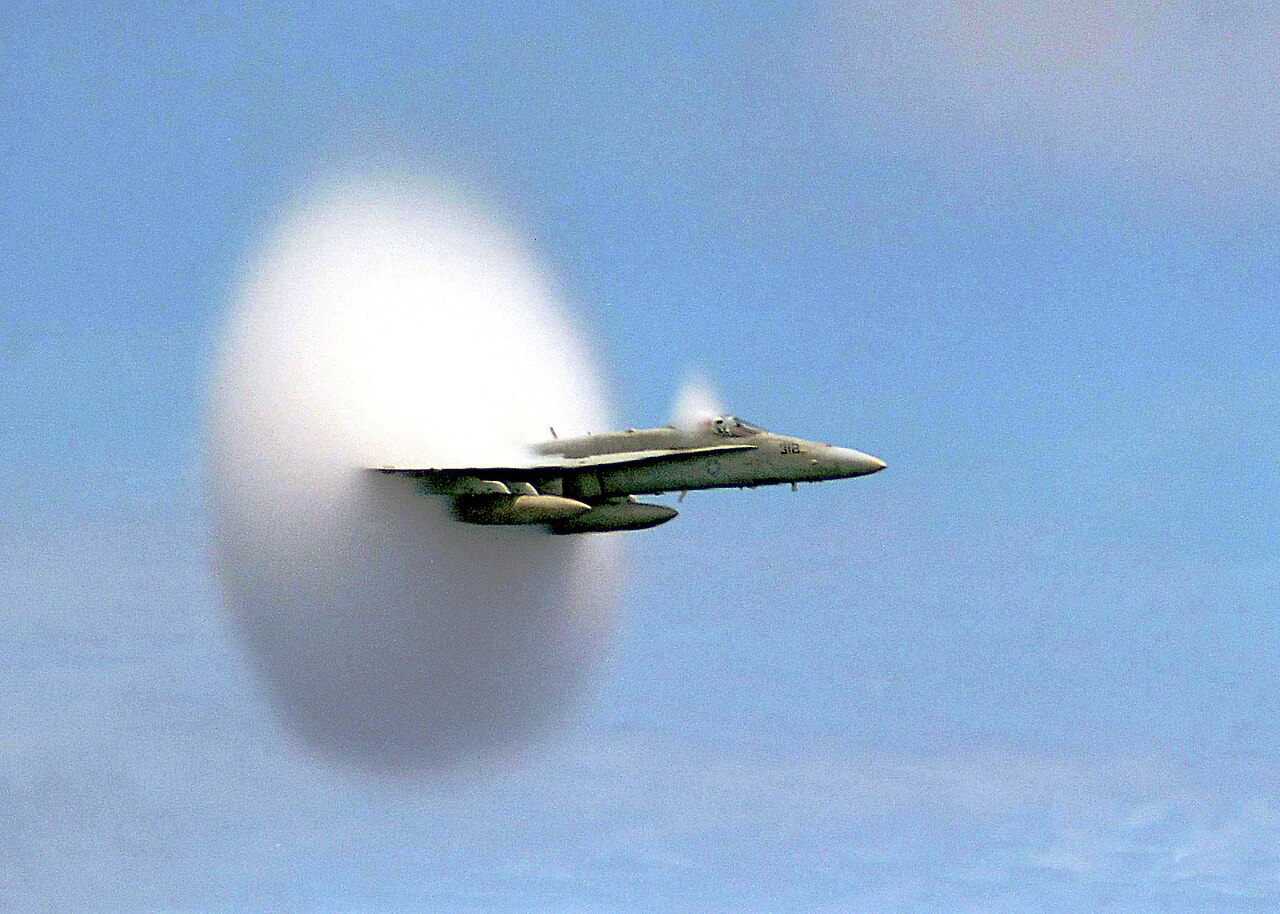
\includegraphics[width=\linewidth]{mach.jpg}
\end{column}

\end{columns}

\end{frame}

\section{Parametry fizyczne}

\subsection{Prędkość dźwięku w powietrzu}

\begin{frame}{Prędkość dźwięku w powietrzu}

	\begin{columns}
		\begin{column}{0.5\textwidth}
			Lab: \pause

			\includegraphics[width=\linewidth]{lab_KlaKop.jpg} \pause
		\end{column}
		\begin{column}{0.5\textwidth}
			Aparatura pomiarowa: \pause
			\begin{itemize}
				\item Miarka 3m \pause
				\item Laptop \pause
				\item Dłonie Franka \pause
				\item Dłonie Jacka \pause
				\item Termometr i higrometr
			\end{itemize}
		\end{column}
	\end{columns}

\end{frame}

\begin{frame}{Zasada działania}

	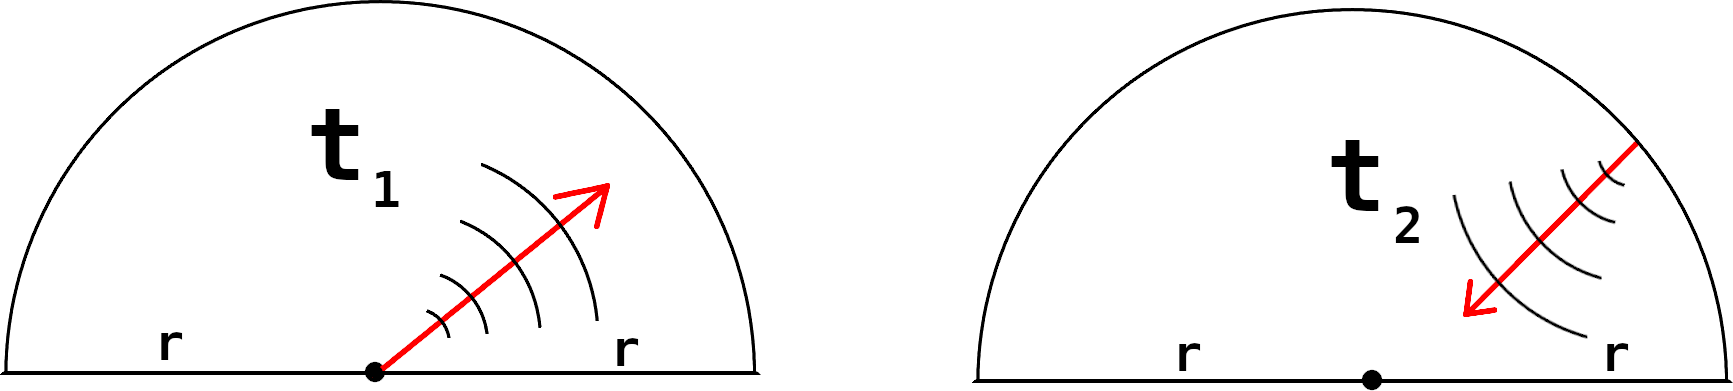
\includegraphics[width=\linewidth]{wave.png}
	$$\Delta t=t_2-t_1$$
	$$v=\frac{2r}{\Delta t}$$

\end{frame}

\begin{frame}{Dane}
	\centering
	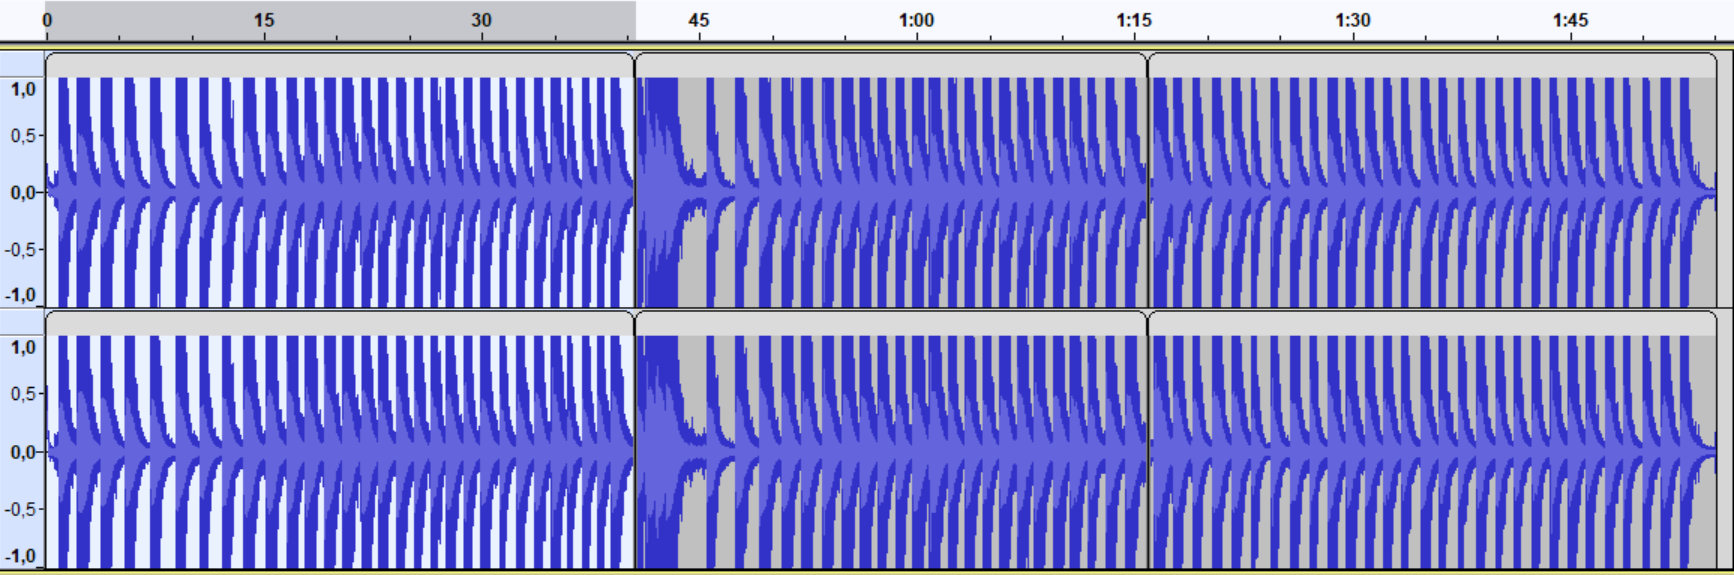
\includegraphics[width=\linewidth]{Data.png} \pause
	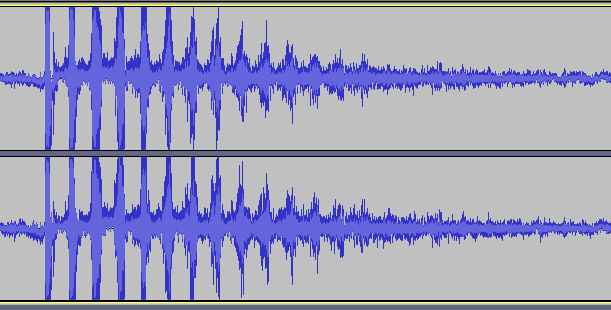
\includegraphics[width=0.7\linewidth]{Przechwycenie obrazu ekranu_2024-05-04_14-41-05.png}
\end{frame}

\begin{frame}{Redukcja danych}
	\centering
	\begin{tabular}{cccc}
		\toprule
		Pomiar & czas [s] & sigma [s] & liczba pomiarów \\
		\midrule
		3      & 0.0534   & 0.00134   & 245             \\
		4      & 0.0533   & 0.00127   & 117             \\
		5      & 0.0544   & 0.00149   & 302             \\
		6      & 0.0548   & 0.00180   & 688             \\
		7      & 0.0550   & 0.00119   & 762             \\
		\bottomrule
	\end{tabular}
	
\pause
	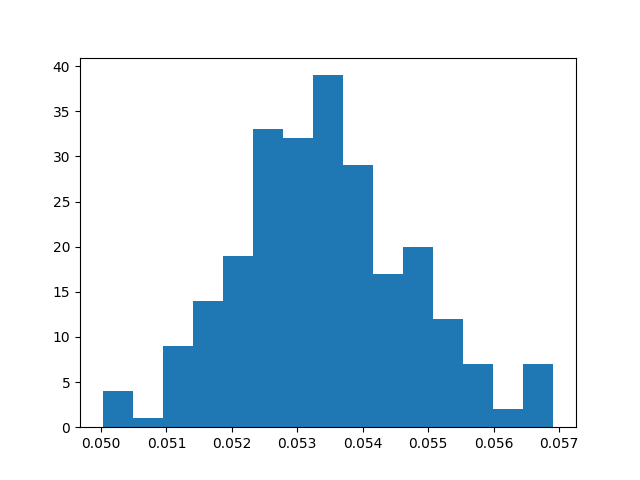
\includegraphics[width=0.2\linewidth]{Hist3.png}
	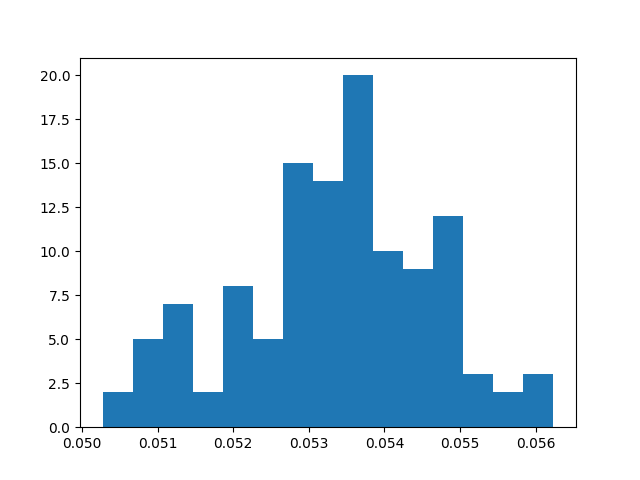
\includegraphics[width=0.2\linewidth]{Hist4.png}
	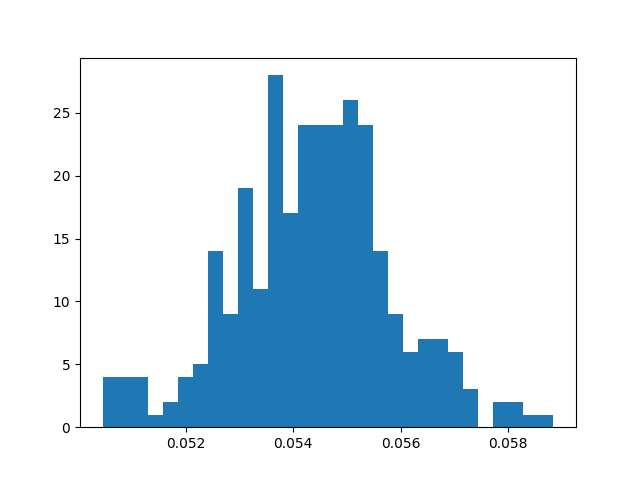
\includegraphics[width=0.2\linewidth]{Hist5.png}
	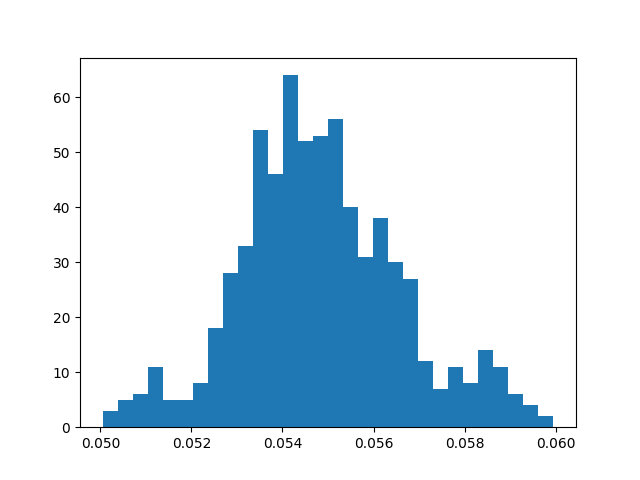
\includegraphics[width=0.2\linewidth]{Hist6.png}
	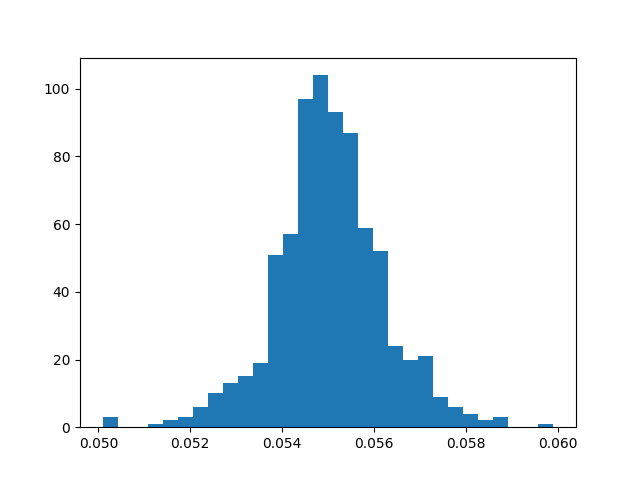
\includegraphics[width=0.2\linewidth]{Hist7.png}
\end{frame}

\begin{frame}{Wyniki i dyskusja błędu pomiarowego}
	\centering
	\begin{tabular}{cccc}
		\toprule
		Pomiar & temperatura [C] & wilgotność [\%] & mach [m/s]       \\
		\midrule
		3      & 29.12           & 27.83           & 355.71$\pm$8.90  \\
		4      & 31.35           & 22.14           & 356.22$\pm$8.51  \\
		5      & 20.22           & 44.42           & 349.41$\pm$9.57  \\
		6      & 18.25           & 51.11           & 346.48$\pm$11.36 \\
		7      & 18.22           & 51.53           & 345.19$\pm$7.46  \\
		\bottomrule
	\end{tabular}

\end{frame}

\begin{frame}{Interpretacja wyników}
	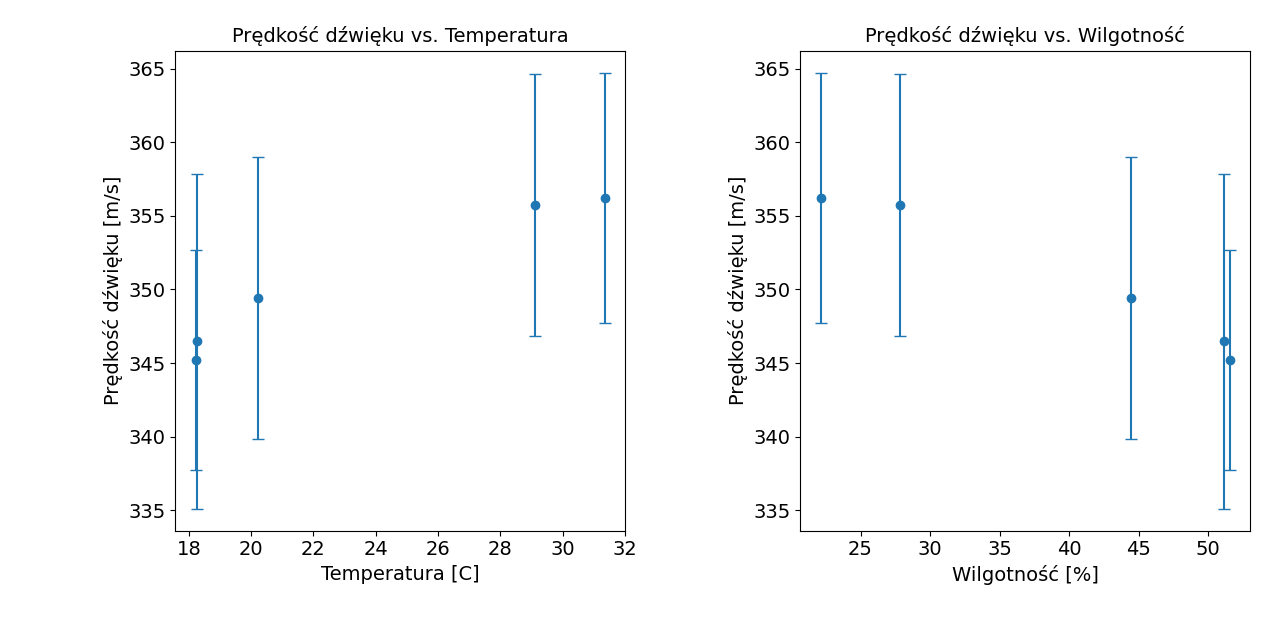
\includegraphics[width=\linewidth]{temp_humid_mach.png}
	Prędkość dźwięku rośnie wraz ze wzrostem temperatury i maleje ze wzrostem wilgotności?
\end{frame}

\section{Stałe matematyczne}

\subsection{$\pi$}

\begin{frame}{$\pi$ - igła Buffona}
	$l=6.5cm$ - długość igły \pause

	$d=8cm$ - odległość między pionowymi liniami \pause

	$n=665$ - liczba rzutów \pause

	$R=334$ - liczba rzutów zakończonych przecięciem \pause

\begin{columns}
\begin{column}{0.5\textwidth}
	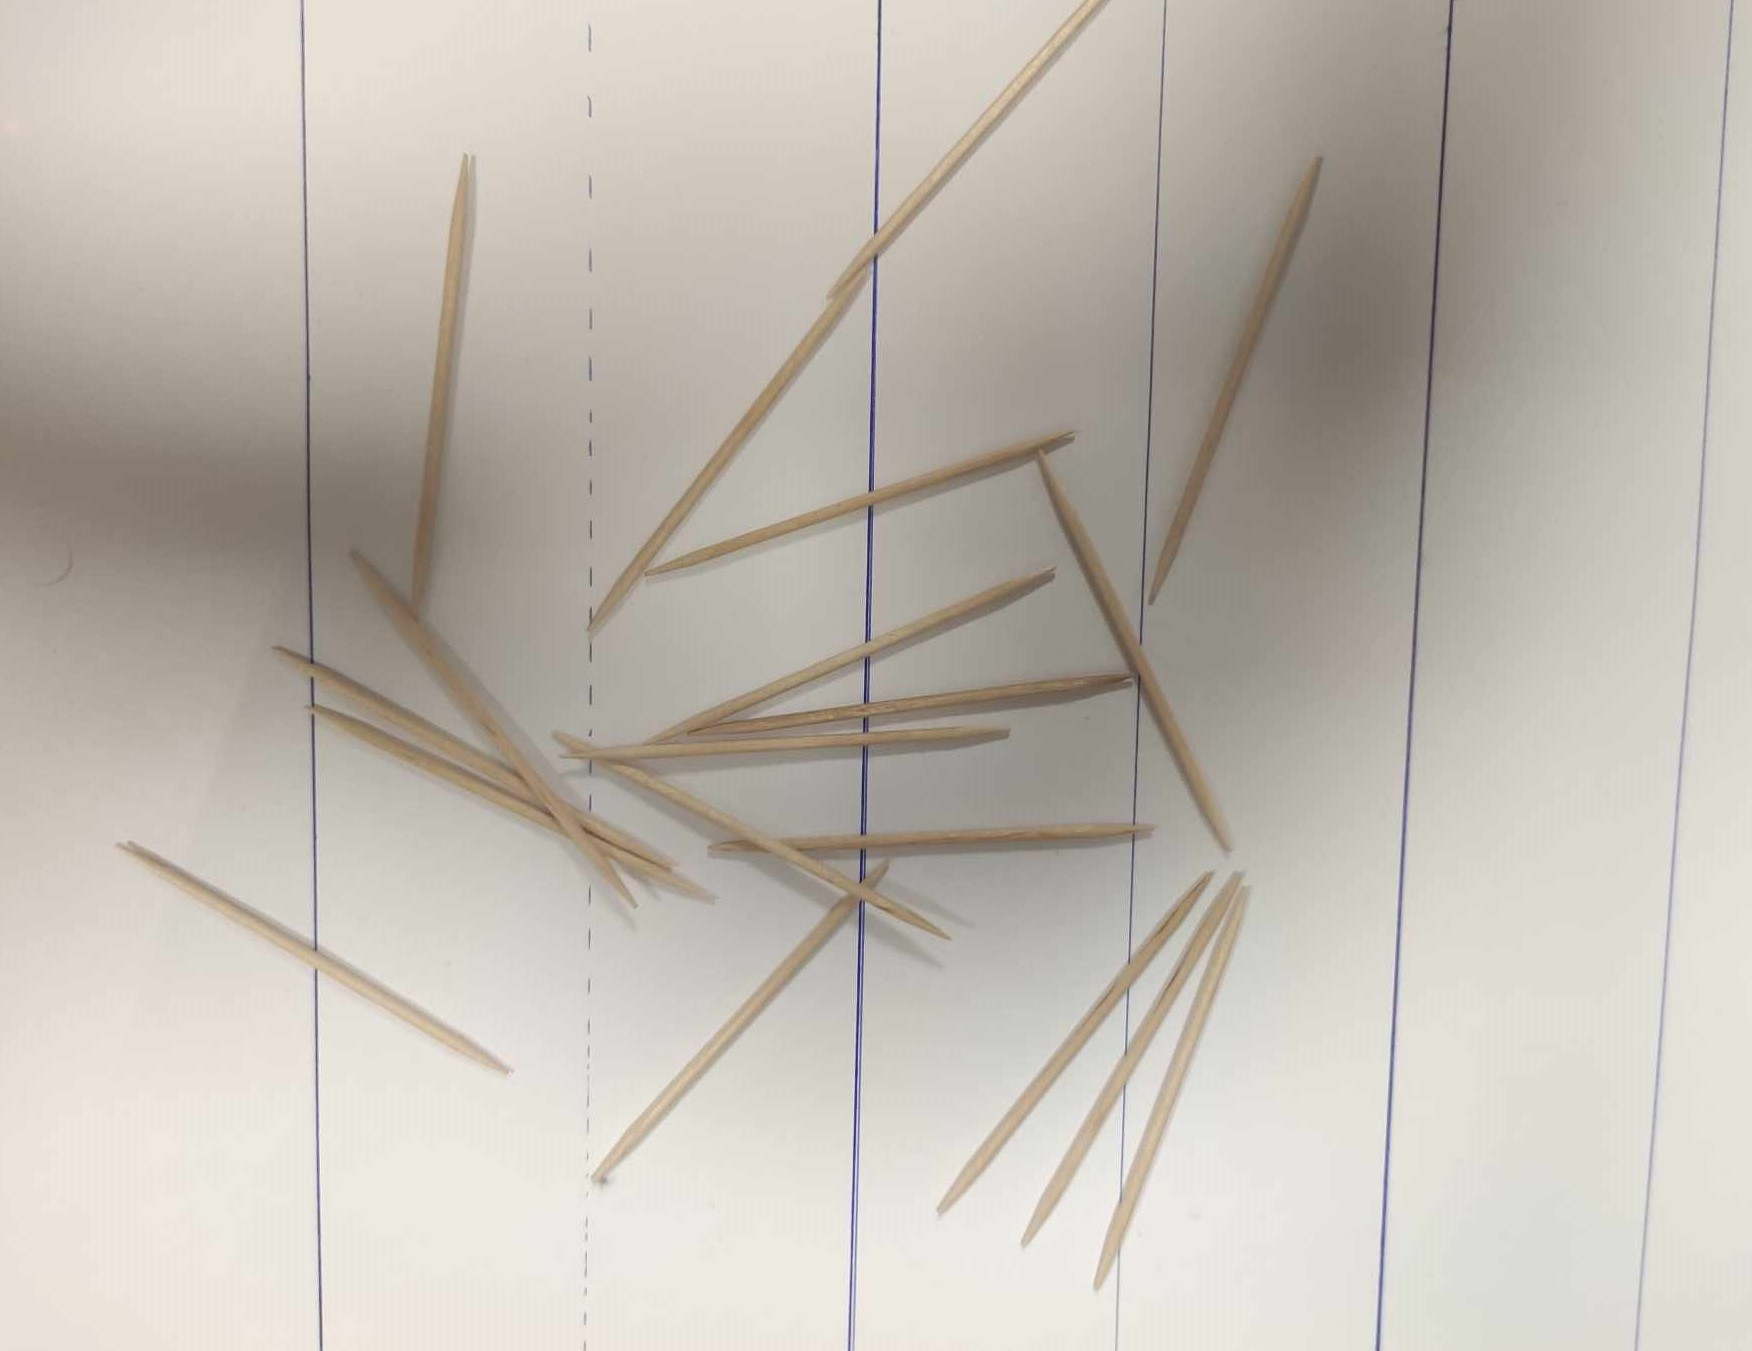
\includegraphics[width=\linewidth]{Buffon.jpg}
\end{column}

\begin{column}{0.5\textwidth}
	$$p = \frac{2}{\pi} \frac{l}{d}$$ \pause
	$$\frac{R}{n} = \frac{2}{\pi}\frac{l}{d}$$ \pause
	$$\pi = \frac{2 l n}{d R}$$ \pause
	$$\pi \approx 3.141$$ \pause
\end{column}

\end{columns}

\end{frame}


\section{Podsumowanie}

\begin{frame}{Dalsze kontynuacje badań}
	\begin{itemize}
		\item $e$
		\item Przenikalność magnetyczna próżni ($\epsilon_0$)
		\item Przenikalność elektryczna próżni ($\mu_0$)
		\item Stała Coulomba ($k_e$)
		\item Prędkość światła ($c$)
		\item Stała Plancka ($h$)
	\end{itemize}

\end{frame}


\end{document}